\documentclass{article}
% Change "article" to "report" to get rid of page number on title page
\usepackage{amsmath,amsfonts,amsthm,amssymb}
\usepackage{setspace}
\usepackage{Tabbing}
\usepackage{fancyhdr}
\usepackage{lastpage}
\usepackage{extramarks}
\usepackage{chngpage}
\usepackage{soul,color}
\usepackage{graphicx,float,wrapfig}
\usepackage{multirow}
\usepackage{enumerate}
% In case you need to adjust margins:
\topmargin=-0.45in      %
\evensidemargin=0in     %
\oddsidemargin=0in      %
\textwidth=6.5in        %
\textheight=9.0in       %
\headsep=0.25in         %

% Homework Specific Information
\newcommand{\hmwkTitle}{Modifications}
\newcommand{\hmwkClass}{}
\newcommand{\hmwkAuthorName}{Donglai\ Wei}


% Setup the header and footer
\pagestyle{fancy}                                                       %
\lhead{\hmwkAuthorName}                                                 %
\rhead{\firstxmark}                                                     %
\lfoot{\lastxmark}                                                      %
\cfoot{}                                                                %
\rfoot{Page\ \thepage\ of\ \pageref{LastPage}}                          %
\renewcommand\headrulewidth{0.4pt}                                      %
\renewcommand\footrulewidth{0.4pt}                                      %

% This is used to trace down (pin point) problems
% in latexing a document:
%\tracingall

%%%%%%%%%%%%%%%%%%%%%%%%%%%%%%%%%%%%%%%%%%%%%%%%%%%%%%%%\begin{enumerate}

% Some tools
\newcommand{\enterProblemHeader}[1]{\nobreak\extramarks{#1}{#1 continued on next page\ldots}\nobreak%
                                    \nobreak\extramarks{#1 (continued)}{#1 continued on next page\ldots}\nobreak}%
\newcommand{\exitProblemHeader}[1]{\nobreak\extramarks{#1 (continued)}{#1 continued on next page\ldots}\nobreak%
                                   \nobreak\extramarks{#1}{}\nobreak}%

\newlength{\labelLength}
\newcommand{\labelAnswer}[2]
  {\settowidth{\labelLength}{#1}%
   \addtolength{\labelLength}{0.25in}%
   \changetext{}{-\labelLength}{}{}{}%
   \noindent\fbox{\begin{minipage}[c]{\columnwidth}#2\end{minipage}}%
   \marginpar{\fbox{#1}}%

   % We put the blank space above in order to make sure this
   % \marginpar gets correctly placed.
   \changetext{}{+\labelLength}{}{}{}}%

\setcounter{secnumdepth}{0}
\newcommand{\homeworkProblemName}{}%
\newcounter{homeworkProblemCounter}%
\newenvironment{homeworkProblem}[1][Problem \arabic{homeworkProblemCounter}]%
  {\stepcounter{homeworkProblemCounter}%
   \renewcommand{\homeworkProblemName}{#1}%
   \section{\homeworkProblemName}%
   \enterProblemHeader{\homeworkProblemName}}%
  {\exitProblemHeader{\homeworkProblemName}}%

\newcommand{\problemAnswer}[1]
  {\noindent\fbox{\begin{minipage}[c]{\columnwidth}#1\end{minipage}}}%

\newcommand{\problemLAnswer}[1]
  {\labelAnswer{\homeworkProblemName}{#1}}

\newcommand{\homeworkSectionName}{}%
\newlength{\homeworkSectionLabelLength}{}%
\newenvironment{homeworkSection}[1]%
  {% We put this space here to make sure we're not connected to the above.
   % Otherwise the changetext can do funny things to the other margin

   \renewcommand{\homeworkSectionName}{#1}%
   \settowidth{\homeworkSectionLabelLength}{\homeworkSectionName}%
   \addtolength{\homeworkSectionLabelLength}{0.25in}%
   \changetext{}{-\homeworkSectionLabelLength}{}{}{}%
   \subsection{\homeworkSectionName}%
   \enterProblemHeader{\homeworkProblemName\ [\homeworkSectionName]}}%
  {\enterProblemHeader{\homeworkProblemName}%

   % We put the blank space above in order to make sure this margin
   % change doesn't happen too soon (else \sectionAnswer's can
   % get ugly about their \marginpar placement.
   \changetext{}{+\homeworkSectionLabelLength}{}{}{}}%

\newcommand{\sectionAnswer}[1]
  {% We put this space here to make sure we're disconnected from the previous
   % passage

   \noindent\fbox{\begin{minipage}[c]{\columnwidth}#1\end{minipage}}%
   \enterProblemHeader{\homeworkProblemName}\exitProblemHeader{\homeworkProblemName}%
   \marginpar{\fbox{\homeworkSectionName}}%

   % We put the blank space above in order to make sure this
   % \marginpar gets correctly placed.
   }%

%%%%%%%%%%%%%%%%%%%%%%%%%%%%%%%%%%%%%%%%%%%%%%%%%%%%%%%%%%%%%



%%%%%%%%%%%%%%%%%%%%%%%%%%%%%%%%%%%%%%%%%%%%%%%%%%%%%%%%%%%%%
% Make title
\title{\vspace{0.3in}\textmd{\textbf{\hmwkTitle}}}
\date{2010.7.11}
\author{\textbf{\hmwkAuthorName}}
%%%%%%%%%%%%%%%%%%%%%%%%%%%%%%%%%%%%%%%%%%%%%%%%%%%%%%%%%%%%%

\begin{document}
\begin{spacing}{1.1}
\maketitle
\section{1)Change of t,k-term: Rescue Annealed Local-Table move}
{\bf Previous Formula}:\\
$-log p(x,z|\lambda)$\\ =\\
(t-term)$ \underline{{\color{red}log \frac{\Gamma(m_{..}+\gamma)}{\Gamma(\gamma)}}+\sum_{j=1}^{J} \{log \frac{\Gamma(n_{j..}+\alpha)}{\Gamma(\alpha)}-\sum_{t=1}^{m_{j.}}[log(\Gamma(n_{jt.}))+log \alpha
]\}}$\\ \\
+(k-term)$ \sum_{k=1}^{K} [log(\frac{\Gamma(n_{..k}+W\phi_{0})}{\Pi_{w=1}^{W}\Gamma(\phi_{0}+n_{..k}^{w})})+log(\frac{\Gamma(\phi_{0})^{W}}{\Gamma(W\phi_{0})})
-\underline{log(\Gamma(m_{.k}))-log \gamma]}$\\ \\
\emph{{\small (underlined part come from Hierarchical Dirichlet Process)}}\\ \\ 
{\bf New Formula}:\\
$-log p(x,z|\lambda)$\\ =\\
(t-term)$ \underline{+\sum_{j=1}^{J} \{log \frac{\Gamma(n_{j..}+\alpha)}{\Gamma(\alpha)}-\sum_{t=1}^{m_{j.}}[log(\Gamma(n_{jt.}))+log \alpha
]\}}$\\ \\
+(k-term)$ \underline{{\color{red}log \frac{\Gamma(m_{..}+\gamma)}{\Gamma(\gamma)}}}+\sum_{k=1}^{K} [log(\frac{\Gamma(n_{..k}+W\phi_{0})}{\Pi_{w=1}^{W}\Gamma(\phi_{0}+n_{..k}^{w})})+log(\frac{\Gamma(\phi_{0})^{W}}{\Gamma(W\phi_{0})})
-\underline{log(\Gamma(m_{.k}))-log \gamma]}$\\ \\ \\ \\
1) Previously,t-term wants only 1 table per restaurant while k-term wants every word forms a dish, which requires subtle annealing schedule.\\ \\
By putting the restriction of $\Gamma(m_{..}+\gamma)$ down to k-term, we now can anneal local-table move avoiding creating too many tables.\\ \\
Annealing Schedule: $[0.2,0.4,0.6,0.8,1]^{p}$\\
Fixing other parameters(p=0.5), Figure 1 is the comparison of the annealing results for different forulae(anneal both local-table and merge-table)\\ \\
2) Other Strategies:\\
i)   no aneal m-t,aneal l-t: doesn't work\\
ii)  aneal m-t,no aneal l-t: WORKS\\
iii) no aneal m-t, no aneal l-t: doesn't work\\ \\
{\bf \{Tests from now on use the new formula\}}
\begin{figure}
 \centering
   \begin{tabular}{cccc}    
     \resizebox{40mm}{!}{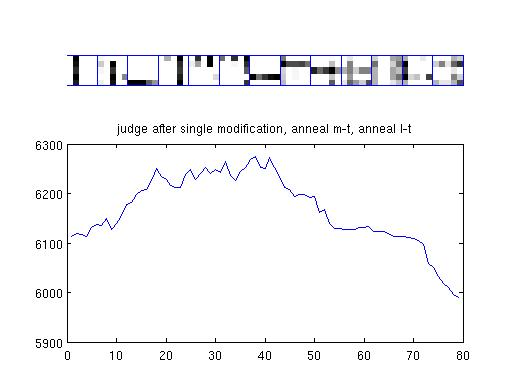
\includegraphics{s_mt_lt.jpg}} &
      \resizebox{40mm}{!}{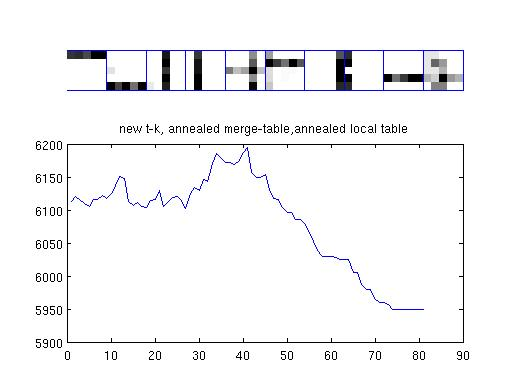
\includegraphics{mt_lt.jpg}}\\ 
        \end{tabular}
    \caption{aneal m-t,aneal l-t   left: Previous t,k-term, right: new t,k-term  }
    \label{fig:by:table} 
\end{figure}
\newpage
\section{2) New merge-table}
1) Previously, in restaurant j, merge-table only tries find the best table $t^{*}$ for certain table t to merge while serving $k_{jt^{*}}$  \\
2) A better merge-table should also search for the best k for the new merged table.\\ \\
Fixing other parameters, Figure 2 is the comparison of the merge-table for different Annealing power p$\in[0.5,1,2]$.\\ \\
{\bf \{Tests from now on use the new merge-table\}}
\begin{figure}
 \centering
   \begin{tabular}{cc}    
      \resizebox{40mm}{!}{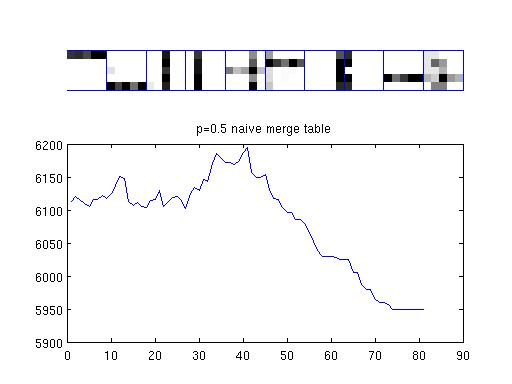
\includegraphics{m_t2_05.jpg}} &
      \resizebox{40mm}{!}{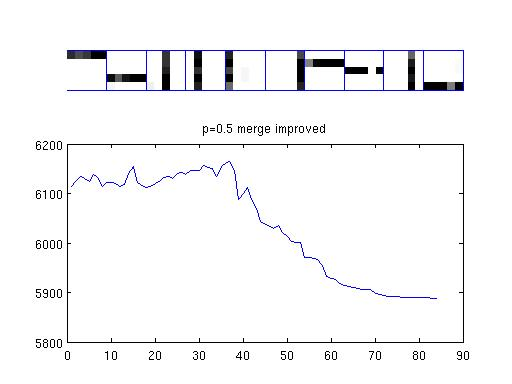
\includegraphics{m_t_05.jpg}} \\ 
      \resizebox{40mm}{!}{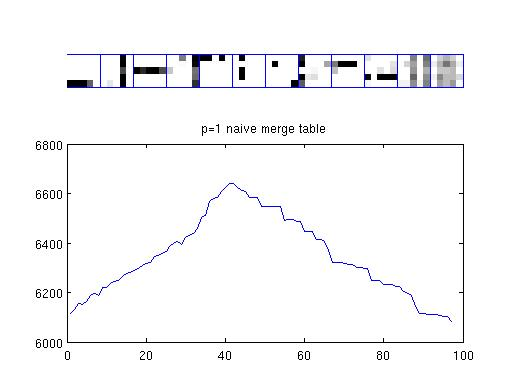
\includegraphics{m_t2_1.jpg}} &
      \resizebox{40mm}{!}{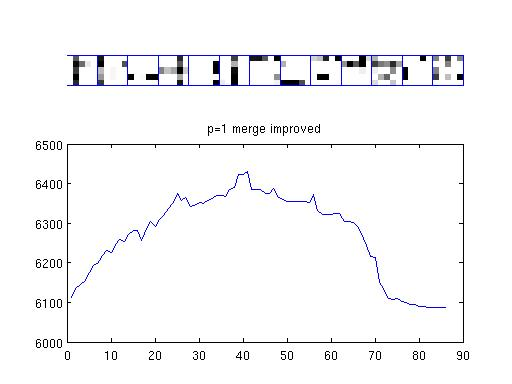
\includegraphics{m_t_1.jpg}} \\ 
      \resizebox{40mm}{!}{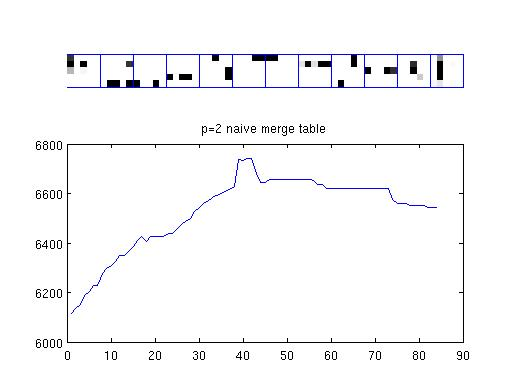
\includegraphics{m_t2_2.jpg}} &
      \resizebox{40mm}{!}{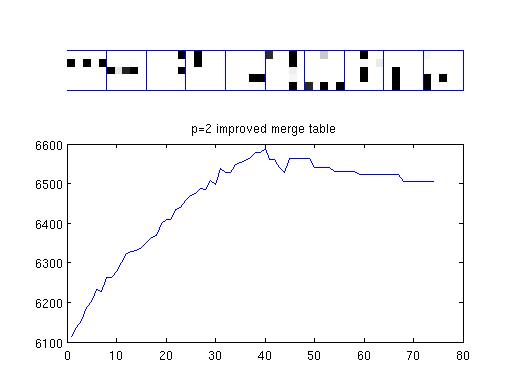
\includegraphics{m_t_2.jpg}} \\ 
    \end{tabular}
    \caption{left: old merge-table; right: new merge-table;   first row: T=0.5; second row: T=1; third row: T=2; }
    \label{fig:by:table} 
\end{figure}

\newpage
\section{3) Local Dish}
\subsection{i) Background}
So far, for tables, we have: \\
1) Local-Table-Refinement\\
2) Local-Search-Dish\\
3) Merge-Table\\ \\
But for dishes, we only have:\\
1) Merge-Dish
\subsection{ii) Local Maxima}
On the left of Figure 3, we expect the third to last dish to be a bar, which shares the word,say w, with the second to last dish.\\ \\
But, in decompose restaurant, we will never see word w magically go to the third to last dish since the (k-term)sampling likelihood is almost 0, while merge-dish is too cumbersome to help.\\ \\
It's not a perfect config since word w in ground truth comes from those two dishes.
In some restaurants, it will cause small tables serving the second to last dish while the third to last dish is around.\\ 
\begin{figure}
 \centering
  \begin{tabular}{cc}    
      \resizebox{40mm}{!}{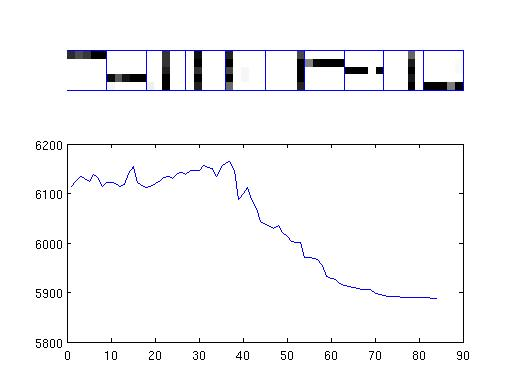
\includegraphics{stuck.jpg}} &
      \resizebox{40mm}{!}{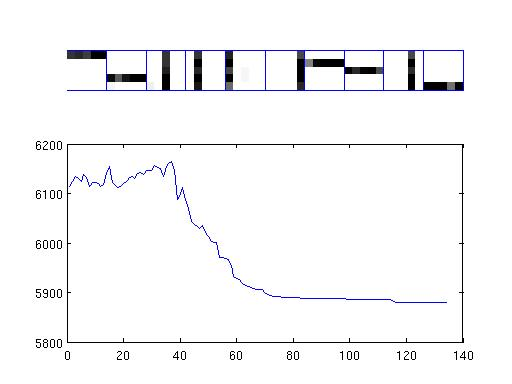
\includegraphics{out.jpg}} \\ 
      \end{tabular}
    \caption{left: Get Stuck; right: Better config by local dish}
    \label{fig:by:table} 
\end{figure}
\subsection{iii) Welcome: Local Dish}
Now we only have the building block "table", which forms restaurants and dishes.\\ \\
There is an another key fundamental part------{\bf Word}\\
We can do Local-Dish-Refinement by greedily deciding the allocation of one certain word in the dish.(exchage it with another dish)\\
(Detail is in the pseudo-code description)
\newpage
\section{4) Remarks}
1) I still think it a bad idea to anneal local-table.\\ \\ Though annealing local-table works for p=0.5(Temperature Schedule:$[0.2,0.4,0.6,0.8,1]^{p}$)\\
It fails(figure 4,left) for p=1,2 while it would still work(figure 4,right) if we do not anneal local-table. Maybe we can make up other stories for it.\\ \\
From Above (p$<$1 is better than others, only anneal merge-table is better than anneal both m-t,l-t), we can see that, we do not need those much annealing to get out of the dominance of t-term. \\ \\
It is only the "merge-table" that is doing bad without annealing, which is too greedy while the dish config is still vague.\\ \\
Also, I did not anneal merge-dish and local-dish, which were doing right things without annealing.\\ \\
If we anneal them, dishes will be less likely to merge or to refine, leading to bad config.
\begin{figure}
 \centering
  \begin{tabular}{cc}    
      \resizebox{40mm}{!}{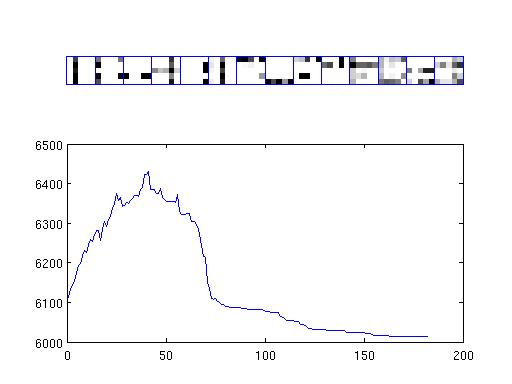
\includegraphics{lt_1.jpg}} &
      \resizebox{40mm}{!}{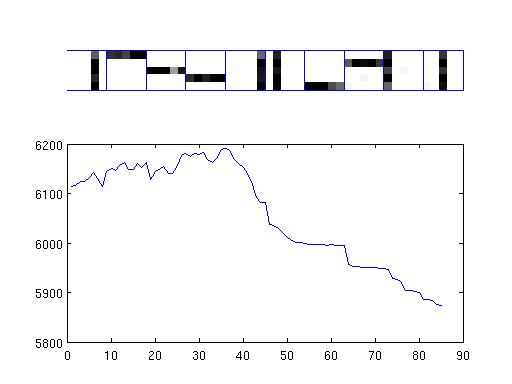
\includegraphics{nlt_1.jpg}} \\ 
      \resizebox{40mm}{!}{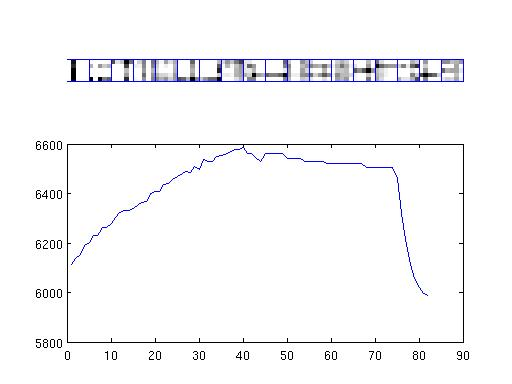
\includegraphics{lt_2.jpg}} &
      \resizebox{40mm}{!}{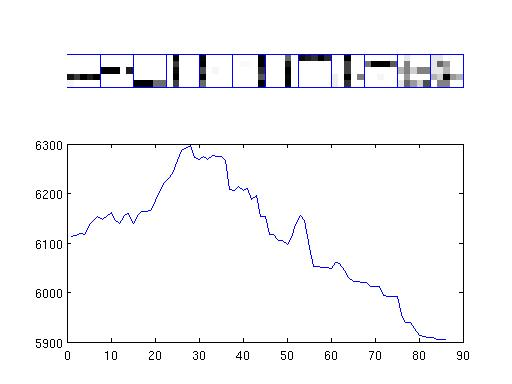
\includegraphics{nlt_2.jpg}} \\       \end{tabular}
    \caption{left: Anneal local-table; right: No Anneal local-table   first row: p=1;second row: p=2; }
    \label{fig:by:table} 
\end{figure}
\newpage
2) Local-Dish move can really make a change:)\\
Above, it seems local-dish is just for further, minor refinement.\\ \\
Figure 5 shows that Local-Dish is {\bf"indispensable"}.\\ \\
I use the same initialization with that from Teh's Gibbs Sampling.(Every Restaurant has 12 tables and there are 12 random flat dish).\\
\begin{figure}
 \centering
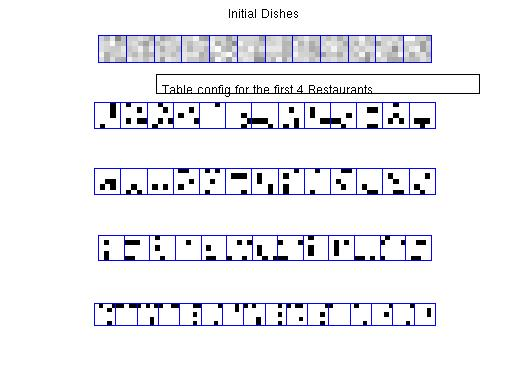
\includegraphics[width=2in,height=2in]{Gibbs_init.jpg}
    \label{fig:by:table} 
\end{figure}

i) We still need annealing, since getting t-term better is a lot easier(simply merge-table) than improving k-term.\\
ii) Again, no anneal local-table is much better \\ 
iii) Without Local-Dish, we can still solve it with other annealing schedule.
But the point is that with Local-Dish, our alogrithm becomes more robust.\\ \\
\begin{figure}
 \centering
  \begin{tabular}{cc}    
      \resizebox{40mm}{!}{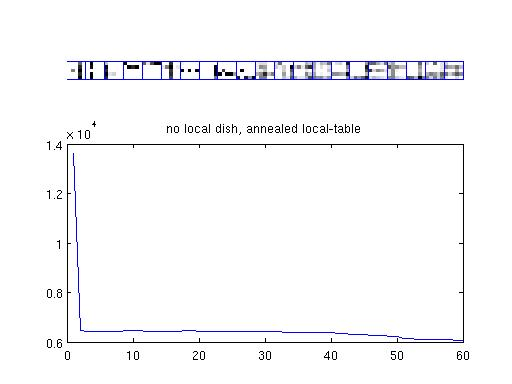
\includegraphics{g_nld_lt.jpg}} &
      \resizebox{40mm}{!}{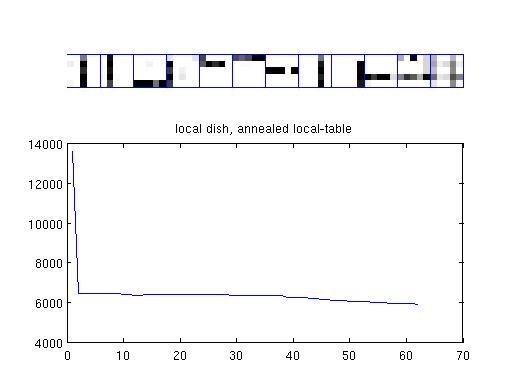
\includegraphics{g_ld_lt.jpg}} \\ 
      \resizebox{40mm}{!}{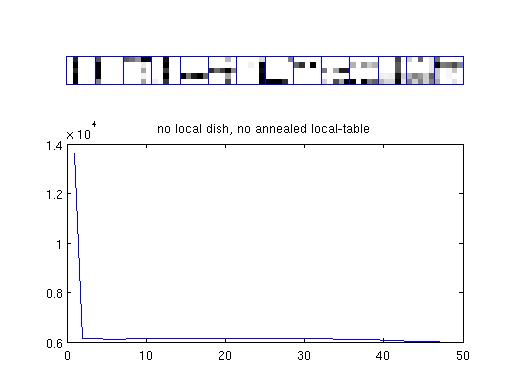
\includegraphics{g_nld_nlt.jpg}} &
      \resizebox{40mm}{!}{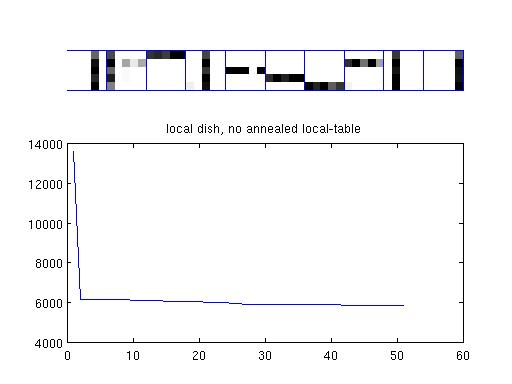
\includegraphics{g_ld_nlt.jpg}} \\       \end{tabular}
    \caption{left: No local-dish; right: local-dish    first row: annealed local-table;second row: no annealed local-table; }
    \label{fig:by:table} 
\end{figure}
3) By now, we've almost figure out for small(40 5 by5 res) and medium(200 5 by5 res) toy data. \\
I'm still debugging mex to see what will happen for larger datas.

\end{spacing}
\end{document}

%%%%%%%%%%%%%%%%%%%%%%%%%%%%%%%%%%%%%%%%%%%%%%%%%%%%%%%%%%%%%
